\documentclass[11pt]{article}
\usepackage{verbatim}
\usepackage{graphicx}
\usepackage{amsmath}
\title{\textbf{Py\_Ellipsoids}}
\author{Ian Merrick\\
		School of Earth and Ocean Sciences\\
		Cardiff University\\
		Wales, UK}
\date{}
\begin{document}

\maketitle

\section{Overview}
The aim of this code is to represent any second order tensor as an ellipsoid for use in virtual globes (i.e. google-earth).

The code is written in python and at its core uses the PyCollada\cite{pycollada} and SimpleKML\cite{simplekml} modules. The code takes a list of defined ellipsoids and creates a zipped KML\cite{kml} file with the ellipsoids embedded as COLLADA\cite{collada} objects.

The code is tested with Python versions $2.7+$ and $3.4+$.

\section{Installation}
Check out the repository from bitbucket\cite{repo}. Assuming you already have python and python-pip installed and in your PATH, you can install all required modules with the command:
\begin{verbatim}
 # pip install -r requirements.txt
\end{verbatim}

\section{Usage}
To run the application, from the command-line type:
\begin{verbatim}
 # python py_ellipsoids.py [-r RESOLUTION] [--keep] input output
\end{verbatim}
where {\em input} is the ellipsoid definition file, {\em output} is the resulting KMZ file, and {\footnotesize RESOLUTION} is the desired resolution of the ellipsoid grid. {\em input} and {\em output} are required arguments, {\footnotesize RESOLUTION} is optional and defaults to $16$. The {\small --keep} option will not remove any of the intermediate collada files.

\section{The Ellipsoid Definition File}
An example ellipsoid definition file is given:
\verbatiminput{../src/ellipsoids_example3.csv}
It is a comma-separated-value (csv) file with headings. The columns of the csv file may be in any order. A list of the required headings are given (with descriptions):
\begin{table}[h]
\begin{tabular}{rl}
 description & (The name or short description of the ellipsoid/tensor)  \\
 A           & (One of the 3 ellipsoid semi-axes lengths (in metres))  \\
 B           & (One of the 3 ellipsoid semi-axes lengths (in metres))  \\
 C           & (One of the 3 ellipsoid semi-axes lengths (in metres))  \\
 lat         & (Global latitude position of the centre of the ellipsoid)  \\
 lon         & (Global longitude position of the centre of the ellipsoid) \\
 alt         & (Altitude of the ellipsoid relative to the ground at lat/lon (in metres))  \\
 alpha       & (Angle in degrees of the pitch of the ellipsoid)  \\
 beta        & (Angle in degrees of the trend of the ellipsoid)  \\
 gamma       & (Angle in degrees of the roll of the ellipsoid)  \\
 colour      & (One of any pre-defined colours)  \\
 transparency& (The level of transparency of the ellipsoid (range 0..1))
\end{tabular}
\end{table}

\noindent The pre-defined set of available colours are listed:
\begin{table}[h]
\begin{tabular}{llllllll}
 white  & silver & grey   & green  & aqua & yellow & olive   & lime   \\
 black  & red    & maroon & teal   & blue & navy   & fuchsia & purple 
\end{tabular}
\end{table}

\subsection{Building the Ellipsoid}
\begin{figure}[h!]
  \caption{An regular icosahedron.}
  \centering
    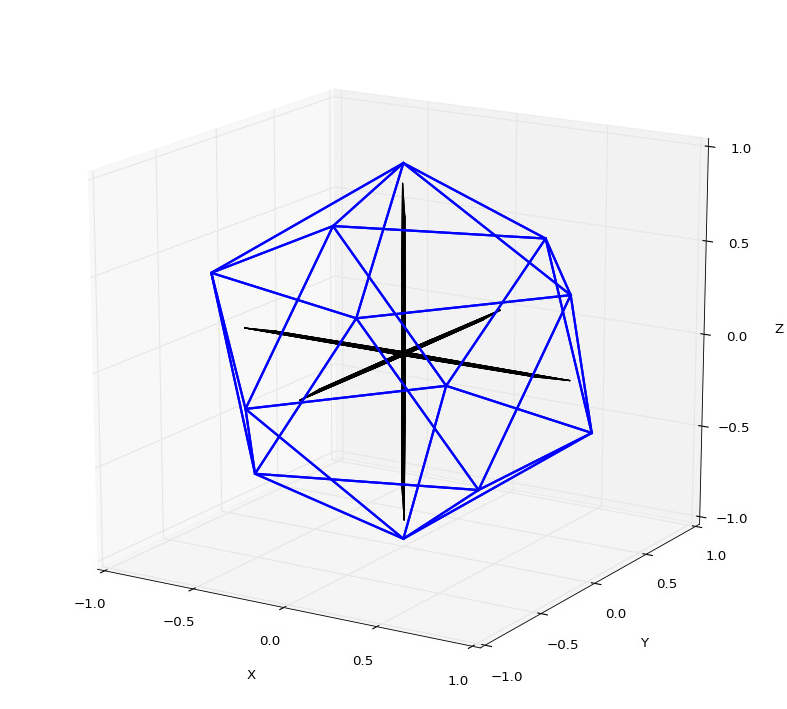
\includegraphics[width=7.5cm]{icosahedron}
    \label{fig:icosahedron}
\end{figure}

Each ellipsoid is built from a regular icosahedron, each radial point normalized to 1.0 (Figure \ref{fig:icosahedron}). To improve resolution, a geodesic grid is created between existing points of the icosahedron, by sub-dividing by {\footnotesize RESOLUTION} points. Figure \ref{fig:icosahedron2_n4} show an icosahedron with an increased number of these geodesic points by  using a {\footnotesize RESOLUTION} of 4.
\begin{figure}[h!]
  \caption{An icosahedron with an increased number of geodesic points using a {\footnotesize RESOLUTION} of 4.}
  \centering
    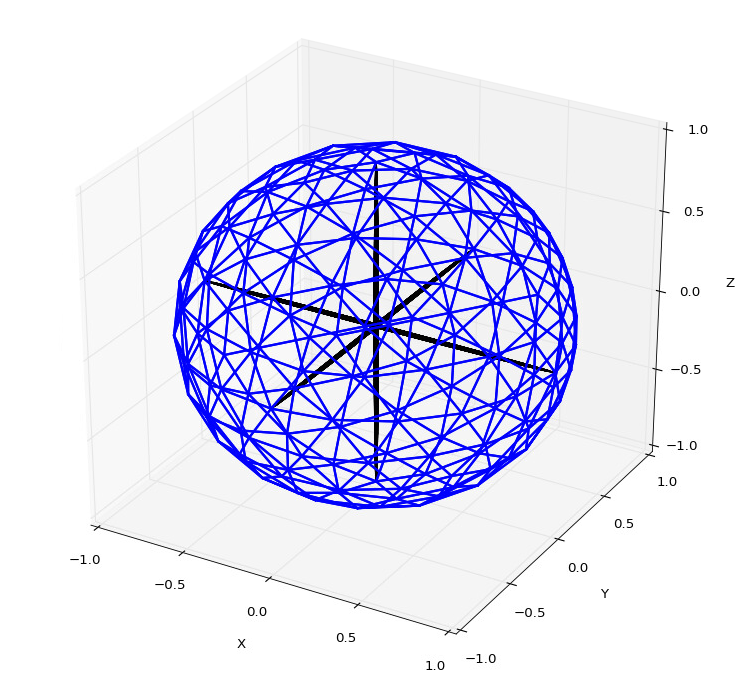
\includegraphics[width=7.5cm]{icosahedron2_n4}
    \label{fig:icosahedron2_n4}
\end{figure}

The icosahedron is then scaled by multiplying the relevant coordinate points by the major, intermediate, and short semi-axis values. In other words, each point p of the sub-divided geodesic icosahedron is scaled as follows:
\begin{equation}
  E_p = 
  \begin{bmatrix}
    S_m I_{p_x} \\
    S_i I_{p_y} \\
    S_s I_{p_z} \\
  \end{bmatrix}
\end{equation}
where $S_m$, $S_i$, and $S_s$ are the lengths of the major, intermediate and minor (short) semi-axes respectively, $I_{p_x}$, $I_{p_y}$, and $I_{p_z}$ are the $xyz$ coordinates of a point $p$ of the geodesic icosahedron, and $E_p$ is the resulting point of the ellipsoid.

\subsection{Position and Orientation of the Ellipsoids}

The convention of the code is to match the X,Y, and Z axes with the local directions of East, North and Up respectively.

The lengths of the three semi-axes of each ellipsoid are provided in the input file (under headings A, B, and C). The order of the listed semi-axes in the input file are not important. The code orientates the ellipsoid, placing the major axis along the X axis (West-East), the intermediate axis along the Y axis (South-North), and the short axis along the Z axis (Up) (Figure \ref{fig:ellipsoids1}).
\begin{figure}[h!]
  \caption{The reference orientation of the ellipsoid.}
  \centering
    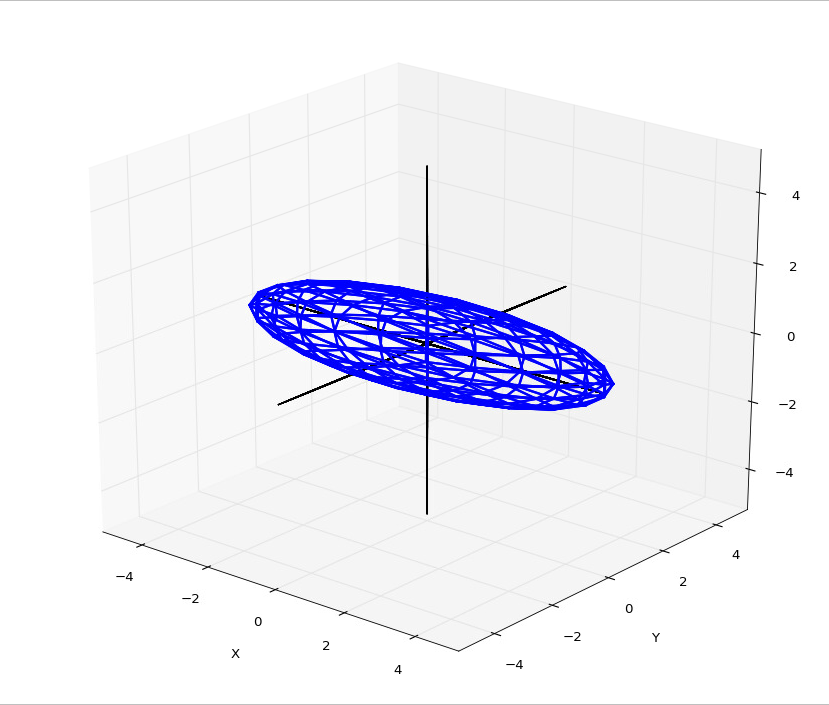
\includegraphics[width=7.5cm]{ellipsoids1}
    \label{fig:ellipsoids1}
\end{figure}

The user defines the orientation of the ellipsoid using the values alpha, beta, and gamma in the input file. These values are rotations in degrees. Rotations are performed about a defined axis and are always rotated anticlockwise as you look down the axis (from a positive viewpoint) towards the origin.

The first rotation is the plunge of the ellipsoid. This is a rotation by alpha degrees about the Y axis. The second rotation is the trend. This is a rotation by beta degrees about the Z axis. The final rotation is the roll. This is a rotation about the major axis of the ellipsoid itself by gamma degrees.


\begin{thebibliography}{1}

  \bibitem{pycollada} PyCollada ({\em https://github.com/pycollada/pycollada}).

  \bibitem{simplekml} SimpleKML ({\em https://code.google.com/p/simplekml}).
  
  \bibitem{kml} KML ({\em http://www.opengeospatial.org/standards/kml}).
  
  \bibitem{collada} COLLADA ({\em https://collada.org/}).
  
  \bibitem{repo} py\_ellipsoids {\em https://bitbucket.org/sglim2/py\_ellipsoids}

\end{thebibliography}

\end{document}
